
\section{Notions de base}

\subsection{Processus DevOps}

Le DevOps désigne une approche organisationnelle et technique visant à rapprocher le développement logiciel et les opérations informatiques afin d’améliorer la rapidité, la fiabilité et la continuité de la livraison logicielle. Il repose notamment sur l’automatisation, l’intégration continue, la livraison continue, la collaboration entre équipes et l’amélioration continue des processus \cite{bass2015devops,leite2020devops}.

Dans ce mémoire, le DevOps constitue le cadre général dans lequel s’inscrit la revue de code. En effet, les modifications de code doivent être conçues, implémentées, vérifiées, révisées puis intégrées avant d’être livrées. La revue de code intervient donc comme une étape de contrôle et de collaboration au sein du cycle de développement logiciel.



\subsection{Pipeline DevOps}

Un pipeline DevOps désigne un enchaînement automatisé et structuré d’étapes permettant de faire évoluer une modification logicielle depuis le code source jusqu’à sa livraison ou son déploiement. Il inclut généralement des phases telles que la compilation, les tests automatisés, l’analyse qualité, la validation, le déploiement et la surveillance. Selon l’organisation du projet, la revue de code peut également constituer une étape préalable à l’intégration des changements dans la branche principale \cite{humble2010continuous,shahin2017continuous}.

L’objectif d’un tel pipeline est de rendre la livraison logicielle plus rapide, fiable et répétable. Toute interruption ou attente prolongée dans l’une de ses étapes peut ralentir le cycle global de livraison.



\subsection{Revue de code}

La revue de code est une activité consistant à examiner le code source produit par un développeur avant son intégration dans la base de code principale. Les inspections formelles de code ont été popularisées par les travaux de Fagan, qui ont montré leur intérêt pour la détection précoce des défauts et la réduction des coûts de correction \cite{fagan1976design}.

Dans les environnements modernes, la revue de code est généralement réalisée de manière outillée et asynchrone à travers des plateformes collaboratives. Elle ne se limite pas à la détection d’erreurs : elle contribue également à améliorer la qualité du code, à assurer le respect des conventions, à favoriser le partage de connaissances et à renforcer la collaboration entre développeurs \cite{bacchelli2013expectations,mcintosh2014impact}.



\subsection{Plateformes de développement collaboratif}

Les plateformes de développement collaboratif, telles que GitHub et GitLab, sont des environnements permettant d’héberger des dépôts logiciels, de gérer l’historique du code source et de coordonner le travail entre développeurs. Elles offrent des fonctionnalités telles que la gestion des branches, le suivi des issues, les requêtes de fusion, les commentaires de revue, les permissions d’accès et, dans certains cas, l’intégration et le déploiement continus.

Ces plateformes jouent un rôle central dans le développement logiciel distribué, car elles fournissent à la fois l’infrastructure technique de gestion du code et les mécanismes de collaboration nécessaires à la revue et à l’intégration des changements \cite{kalliamvakou2014promises,github_about_pr,gitlab_merge_requests}.



\subsection{Logiciel à code source ouvert}
Un logiciel à code source ouvert, ou open source, est un logiciel dont les conditions de distribution permettent l’accès au code source, sa redistribution et la création de versions modifiées. Selon l’Open Source Initiative, l’accès au code source ne suffit pas à lui seul : la licence doit également autoriser la redistribution et les travaux dérivés selon des conditions compatibles avec la définition de l’open source. Dans ce mémoire, cette notion est importante à deux niveaux : d’une part, RevMine est développé comme une plateforme à code source ouvert ; d’autre part, les projets open source constituent des sujets d’étude privilégiés pour la collecte et la validation expérimentale \cite{osi_osd}.


\subsection{Requête de fusion (Pull Request / Merge Request)}

Une requête de fusion (Pull Request sur GitHub ou Merge Request sur GitLab) est un mécanisme permettant à un développeur de proposer l’intégration de ses modifications dans une branche cible.

Comme le décrivent \cite{gousios2014exploratory}, elle constitue le support principal du modèle de développement basé sur les contributions (pull-based development), en centralisant les modifications de code, l’historique des commits, ainsi que les discussions et commentaires associés. Elle est ainsi au cœur du processus de revue de code moderne.

\subsection{Cycle de vie d’une requête de fusion}
\begin{figure}[H]
\centering
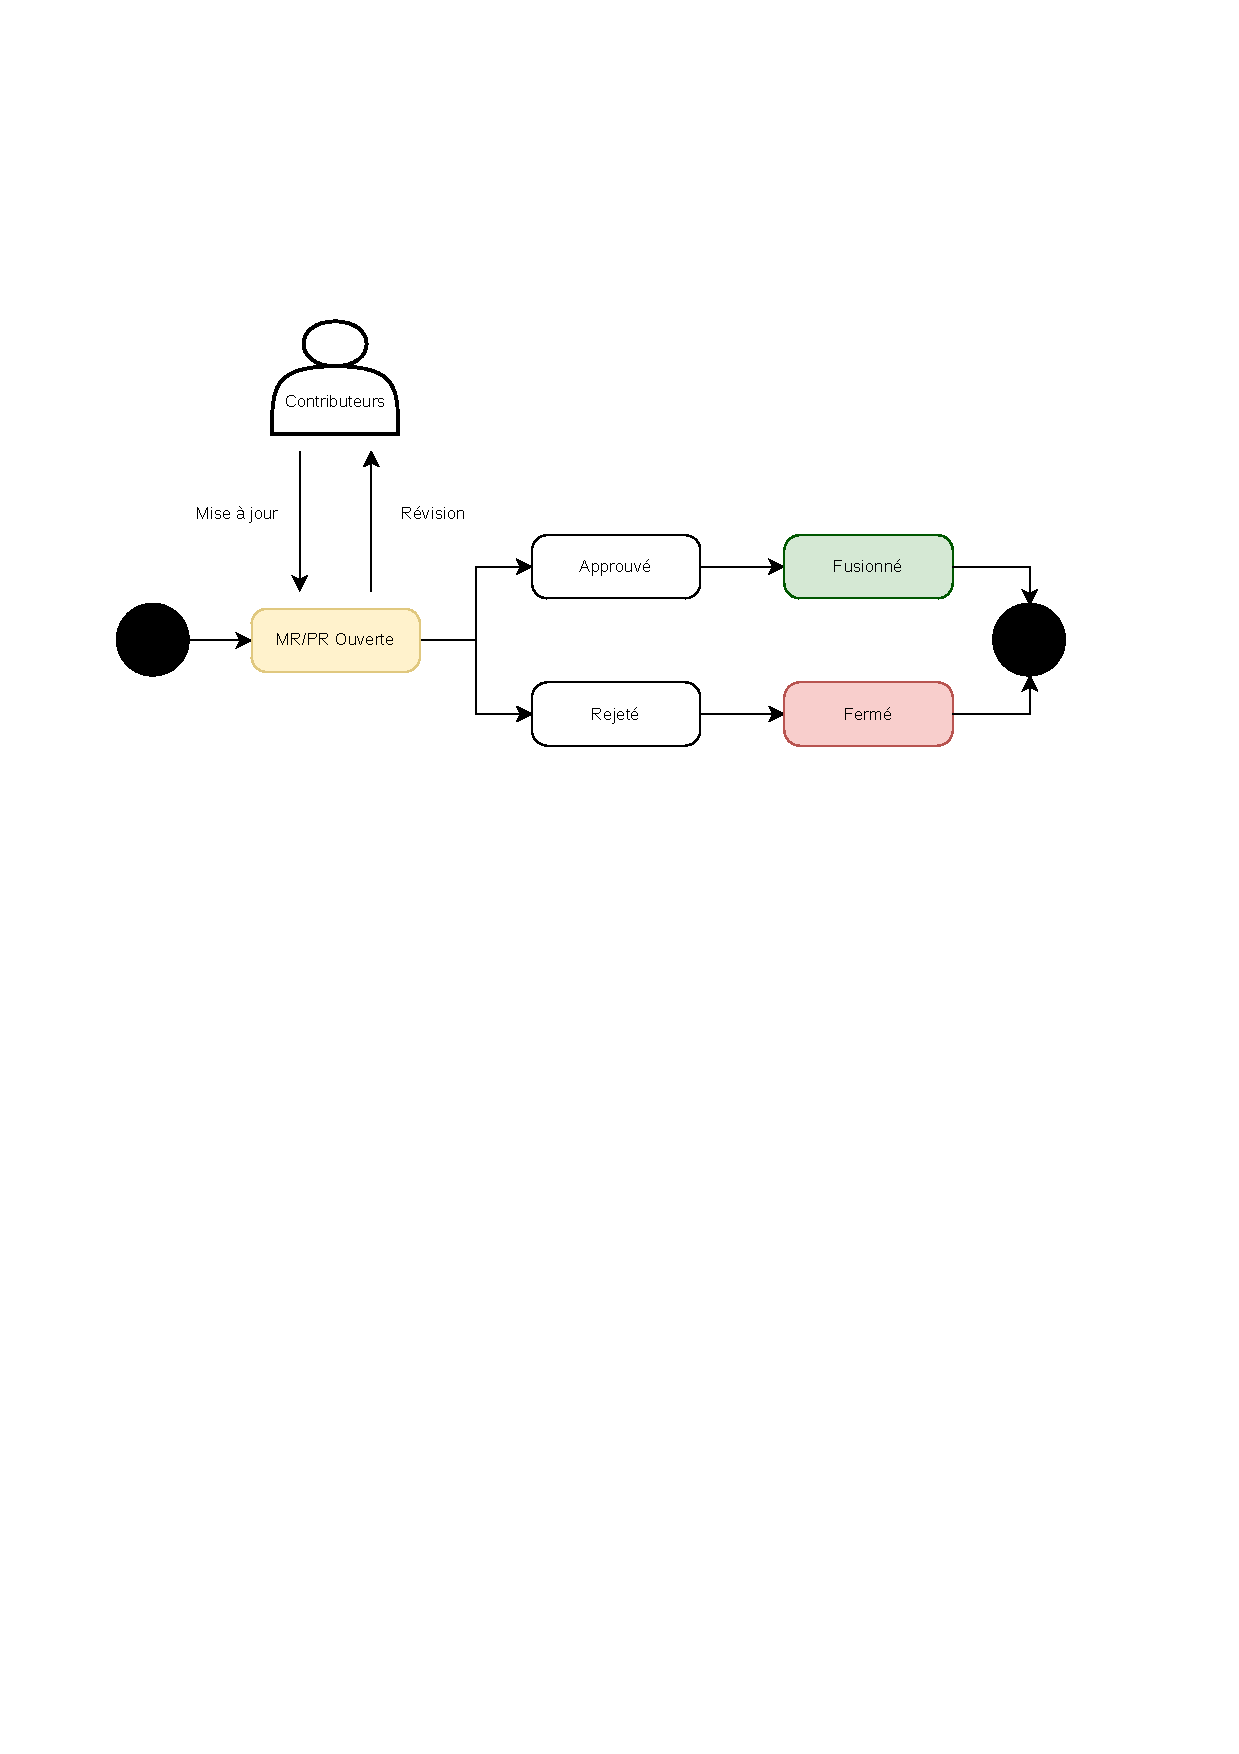
\includegraphics[width=0.8\textwidth, height=0.6\textheight, keepaspectratio]{figures/diag-mrlc (1).pdf}
\caption{\label{fig:lc}Cycle de vie d’une requête de fusion}
\end{figure}
Dans ce mémoire, nous considérons le cycle de vie d’une requête de fusion tel qu’illustré à la figure \ref{fig:lc}. Une requête de fusion peut passer par plusieurs états :

\begin{itemize}
\item \textbf{Ouverte :} Il s’agit de l’état initial au moment de la création d’une requête de fusion. Cet état indique que la requête est disponible pour révision et discussion.
\item \textbf{Fermée :} La requête a été clôturée sans qu’une fusion ait été effectuée. Cela peut se produire lorsque les modifications proposées ne sont plus nécessaires, jugées inappropriées ou lorsque certains problèmes ne peuvent pas être résolus.

\item \textbf{Fusionnée :} Les changements proposés ont été validés et intégrés dans la branche cible. Le code est désormais inclus dans la base de code principale.

\item \textbf{Autres états :} Dans certains cas, les développeurs marquent leurs requêtes comme « Work In Progress (WIP) » ou « brouillon » afin de partager l’avancement de leur travail sans solliciter immédiatement une révision.
\end{itemize}

\subsection{Commit}

Un commit est une unité d’enregistrement dans l’historique d’un dépôt Git. Il représente un ensemble cohérent de modifications appliquées à un ou plusieurs fichiers, accompagné d’un message décrivant les changements réalisés. Chaque commit possède un identifiant unique, généralement appelé hash ou SHA, qui permet de le retrouver dans l’historique du projet \cite{github_about_commits}.

Dans le contexte des revues de code, les commits associés à une requête de fusion permettent d’analyser l’évolution des changements proposés, le volume de code modifié et le rythme de contribution.



% \begin{figure}
% \centering
% \includegraphics[width=0.8\textwidth, height=0.6\textheight, keepaspectratio]{figures/diag-mrlc.pdf}
% \caption{\label{fig:lc}Cycle de vie d’une requête de fusion}
% \end{figure}

\subsection{Acteurs de la revue de code}

Comme le montre la figure \ref{fig:mc}, plusieurs acteurs interviennent dans le processus de revue d’une requête de fusion afin d’en assurer l’efficacité et la qualité :

\begin{itemize}
\item \textbf{Auteur :} Le développeur qui a soumis les modifications et créé la requête de fusion. Il est chargé d’envoyer les demandes de révision et de répondre aux commentaires formulés par les réviseurs.

\item \textbf{Contributeurs (Committers) :} Ce groupe regroupe les membres de l’équipe travaillant sur les changements proposés, y compris l’auteur. Ils sont responsables des mises à jour successives du code.

\item \textbf{Réviseurs :} Les personnes en charge d’examiner le nouveau code afin d’en évaluer la qualité, la cohérence et la conformité. Ils échangent avec les contributeurs pour proposer des corrections ou des améliorations.

\item \textbf{Commentateurs :} Tous les participants (auteurs, contributeurs, réviseurs ou autres intervenants) qui laissent des commentaires pour discuter des modifications apportées. GitLab permet également à des bots d’ajouter des commentaires automatiques pour fournir des informations standardisées.

\item \textbf{Intégrateur :} L’individu chargé de décider si la requête doit être fusionnée, rejetée ou encore modifiée. Ce rôle peut être tenu par l’auteur ou un autre membre de l’équipe de contributeurs.

\end{itemize}

\begin{figure}[H]
\centering
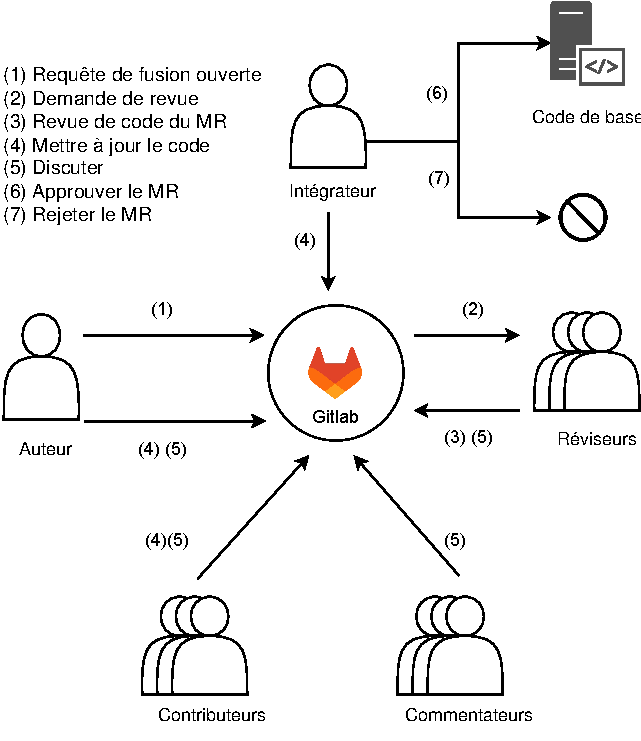
\includegraphics[width=0.8\textwidth, height=0.4\textheight]{figures/diag-Mrm (1).pdf}
\caption{\label{fig:mc}Mécanisme d’interaction autour d’une requête de fusion}
\end{figure}



\subsection{Goulot d’étranglement en revue de code}

Un goulot d’étranglement désigne un point de ralentissement qui limite la progression globale d’un processus. Dans un contexte DevOps, la revue de code peut devenir un goulot d’étranglement lorsque les requêtes de fusion restent en attente trop longtemps, lorsque les réviseurs ne sont pas disponibles ou lorsque les échanges nécessaires à la validation prennent un temps excessif.

Ces ralentissements peuvent retarder l’intégration des changements et affecter la vitesse de livraison. Des travaux récents montrent que le temps de réaction et le temps jusqu’à la fusion sont des préoccupations importantes pour les praticiens, car ils influencent directement la vélocité du développement \cite{kudrjavets2024speed}. D’autres travaux ont également montré que la couverture et la participation dans la revue de code sont liées à la qualité logicielle \cite{mcintosh2014impact}.





\subsection{Métriques en ingénierie logicielle}

Les métriques logicielles sont des indicateurs quantitatifs utilisés pour évaluer les processus et les produits logiciels.  \cite{fenton2014software} soulignent qu’elles doivent être valides, fiables et exploitables.

Avec l’évolution du génie logiciel, l’utilisation de métriques est devenue essentielle pour améliorer les pratiques DevOps. Les métriques DORA (DevOps Research and Assessment) ont été largement adoptées comme référence pour évaluer la performance des équipes.

Cependant, des métriques plus spécifiques sont aujourd’hui utilisées pour analyser des aspects précis, notamment la revue de code. Dans ce contexte, on s’intéresse à des indicateurs tels que le temps de revue (lead time), l’engagement des réviseurs ou encore le volume de modifications (code churn).

\subsection{Ingénierie logicielle empirique et Mining Software Repositories}

L’ingénierie logicielle empirique est une approche de recherche qui étudie les produits, les processus et les pratiques du développement logiciel à partir d’observations, de mesures et de données issues de projets réels. Elle permet de formuler, vérifier ou nuancer des conclusions sur le fonctionnement effectif des équipes et des systèmes logiciels.

Dans ce cadre, le Mining Software Repositories consiste à exploiter les données provenant de dépôts logiciels et de plateformes de développement afin d’extraire des connaissances sur l’évolution du code, la collaboration, la qualité logicielle et les processus de développement. Les travaux de ce domaine soulignent l’importance de protocoles de collecte et d’analyse systématiques afin de garantir la validité et la reproductibilité des résultats \cite{hassan2008road,vidoni2022systematic}.

% \subsection{Jeu de données}

% Un jeu de données, ou dataset, désigne un ensemble organisé de données collectées, structurées et préparées en vue d’être analysées, partagées ou réutilisées. Dans ce mémoire, un jeu de données de revue de code regroupe des informations extraites depuis GitHub ou GitLab, telles que les requêtes de fusion, les commits, les commentaires, les dates de création, de fermeture ou de fusion, les auteurs, les réviseurs et les fichiers modifiés.

% La qualité d’un jeu de données dépend de plusieurs facteurs, notamment la complétude des informations collectées, la cohérence des formats, la traçabilité de la collecte et la documentation des métadonnées associées \cite{datacite_metadata_2024}.



Dans ce mémoire, cette notion est importante à deux niveaux. D’une part, RevMine est développé comme une plateforme à code source ouvert. D’autre part, les projets open source constituent des sujets d’étude privilégiés pour la collecte, l’analyse et la validation expérimentale des données de revue de code.

\subsection{Intelligence artificielle générative}

L’intelligence artificielle générative désigne une catégorie de systèmes capables de produire du contenu, tel que du texte, du code, des images ou des structures de données, à partir de modèles appris sur de grands volumes de données. Cette famille de systèmes s’appuie notamment sur des modèles de fondation capables d’être adaptés à plusieurs tâches en aval \cite{bommasani2021foundation}.

Dans le domaine du génie logiciel, l’intelligence artificielle générative est de plus en plus utilisée pour assister certaines activités telles que la génération de code, la documentation, l’aide à la compréhension de programmes, l’analyse de requêtes utilisateur et l’automatisation partielle de tâches de développement \cite{hou2024llmse}.

\subsection{Modèles de langage}

Les grands modèles de langage, ou Large Language Models (LLMs), sont des modèles d’intelligence artificielle entraînés sur de très grands corpus textuels et capables de traiter, générer et transformer du langage naturel. Certains modèles sont également entraînés ou adaptés sur du code source, ce qui leur permet d’être utilisés dans des tâches de génie logiciel \cite{brown2020language,hou2024llmse}.

Dans le contexte de RevMine, les modèles de langage ne remplacent pas les services de collecte ou d’analyse. Ils servent plutôt de couche d’assistance permettant d’interpréter des besoins exprimés en langage naturel et de les transformer en configurations structurées exploitables par la plateforme.

\subsection{Analyse des données de revue de code}

L’analyse des données de revue de code consiste à exploiter les informations produites par les plateformes collaboratives afin de comprendre, mesurer et améliorer les pratiques de revue. Ces informations peuvent inclure les requêtes de fusion, les commits, les commentaires, les approbations, les dates, les auteurs, les réviseurs, les fichiers modifiés et les métadonnées associées.

Cette analyse permet d’étudier des aspects tels que les délais de revue, la charge des réviseurs, l’engagement des participants, le volume de modifications, les zones fréquemment modifiées et les points de ralentissement du processus. Elle s’inscrit ainsi dans une démarche d’ingénierie logicielle empirique et de Mining Software Repositories, où les décisions d’amélioration sont fondées sur des données observables plutôt que sur des impressions subjectives \cite{bacchelli2013expectations,gousios2014exploratory,vidoni2022systematic}.



\section{Étude de literature sur la revue de code}

La revue de code représente une composante essentielle du processus d’amélioration logicielle. De nombreuses recherches ont mis en évidence son rôle déterminant dans la garantie de la qualité du code et la fiabilité des produits logiciels \parencite{tufano2021towards, oh2005reflective}. Elle contribue non seulement à la détection précoce des anomalies, mais aussi à l’amélioration continue des pratiques de développement \parencite{mcintosh2014impact, bavota2015four}.

Plusieurs travaux se sont attachés à identifier les facteurs qui influencent le déroulement et l’efficacité des revues, notamment ceux liés à la qualité du code et aux dynamiques de collaboration entre développeurs \parencite{kononenko2016code, dougan2022towards}.

Toutefois, la dépendance à l’intervention humaine rend le processus sujet à divers aléas : comportements inattendus \parencite{fuggetta2000software}, retards parfois significatifs — pouvant atteindre plusieurs heures \parencite{bosu2013impact} — et variations dans la qualité des révisions \parencite{dougan2022towards}.
Face à ces limites, la communauté scientifique a proposé diverses approches visant à automatiser, rationaliser et optimiser la revue de code afin d’en renforcer la rigueur et l’efficacité.

\subsection{Automatisation de la revue de code}
Pour automatiser le processus de revue de code, \textcite{tufano2021towards} se concentre sur l’amélioration simultanée des rôles du contributeur et du réviseur. Leur approche repose sur deux architectures d’apprentissage profond distinctes, entraînées à partir de scénarios réels de revues de code. Le modèle proposé suggère des modifications à l’auteur avant la soumission officielle, et propose également aux réviseurs des commentaires inspirés de situations similaires déjà rencontrées. Cette méthode a permis d’obtenir 16 \% de suggestions pertinentes du côté des contributeurs et une amélioration de 31 \% du côté des réviseurs.

De leur côté, \textcite{gupta2017deepfix} ont introduit un modèle séquence-à-séquence à plusieurs couches capable d’identifier et de corriger de manière itérative les erreurs présentes dans des programmes écrits en C. Leur approche a réussi à automatiser la correction de 27 \% des échantillons de test. De façon similaire, \textcite{chen2019sequencer} ont développé un modèle destiné à corriger automatiquement les bogues à une seule ligne dans le code Java ; leur meilleure configuration a atteint une précision de 20 \% sur les exemples testés. D’autres travaux se sont intéressés à la complétion de code afin de générer du code correct et prévenir l’introduction d’erreurs \cite{sadovykh2021veridevops, alon2020structural}.

Dans un contexte industriel, l'automatisation de la revue de code demeure un défi complexe en raison de la diversité des environnements de développement, de la fréquence élevée des demandes de revue, de la taille considérable des projets logiciels et de la variabilité des processus entre équipes. Plusieurs études ont proposé des solutions adaptées à ces contraintes. Par exemple, \textcite{kim2022understanding} ont conçu un bot de revue de code pour Samsung Electronics, capable de mesurer la taille des changements soumis, de détecter les fautes de frappe, les défauts potentiels et les violations de style. Les ingénieurs de l’entreprise ont exprimé leur satisfaction face à cet outil, qui leur permet d’accélérer significativement les révisions.

De même, Google a mis au point un système d’analyse et de revue de code intégré à son flux de développement \cite{sadowski2015tricorder, potvin2016google}, tandis que Microsoft a adopté divers outils d’assurance qualité effectuant des analyses automatisées du code \cite{bird2015lessons}. Ces systèmes, bien qu’efficaces, ne suppriment toutefois pas totalement la nécessité d’une intervention humaine dans le processus de revue.

\subsection{Explication du processus de revue de code à l’aide de modèles d’apprentissage automatique}

Les travaux portant sur l’automatisation de la revue de code montrent qu’une automatisation complète du processus reste impossible et nécessitera toujours une intervention humaine. Face à cette limite, plusieurs recherches se sont orientées vers l’utilisation de l’apprentissage automatique afin de mieux comprendre l’influence de divers indicateurs associés aux revues, dans le but d’en améliorer l’efficacité et la rapidité.

Par exemple, \textcite{chouchen2023learning} ont conçu un modèle d’apprentissage automatique capable de prédire le temps nécessaire à la finalisation d’une revue de code, tout en identifiant les facteurs qui influencent cette durée. \textcite{hasan2023understanding} ont montré qu’un délai de première réponse plus court — qu’elle provienne d’un bot ou d’un humain — est généralement associé à une durée de revue plus brève. Toutefois, cette corrélation ne se vérifie pas toujours dans les cas où les bots initient la première interaction, en raison d’une moindre implication des développeurs.

Selon \textcite{bosu2014impact}, les développeurs expérimentés reçoivent un retour initial plus rapide, ce qui se traduit par une réduction du temps global de revue. \textcite{jiang2013will} ont quant à eux démontré que le nombre de réviseurs influe sur la durée du processus. De plus, \textcite{thongtanunam2017review} se sont intéressés aux caractéristiques des correctifs de code qui attirent un plus grand nombre de réviseurs.
D’autres études, telles que celles de \textcite{li2020redundancy} et \textcite{khatoonabadi2023wasted}, se sont penchées sur les demandes de fusion dupliquées ou abandonnées, qui mobilisent inutilement le temps et les efforts des développeurs. Enfin, \textcite{fan2018early} et \textcite{islam2022early} ont proposé des approches permettant de prédire, dès les premières étapes, si les modifications proposées seront intégrées dans la base de code principale.

Dans le contexte industriel, plusieurs études ont également tenté d’expliquer et d’optimiser le processus de revue de code. Chez Microsoft, par exemple, \textcite{maddila2023nudge} ont proposé un modèle capable de prédire la durée des revues, de détecter les activités et d’identifier les acteurs responsables des blocages dans les demandes de fusion. \textcite{hasan2021using} ont présenté une approche globale visant à évaluer et prédire la qualité des revues tout en abordant les défis rencontrés par les réviseurs.
De leur côté, \textcite{wang2019leveraging, wang2021large} ont formulé le problème de l’estimation de l’effort de revue comme une tâche de classification binaire, définissant les revues exigeant un effort important comme celles ayant nécessité plus de deux itérations de correction chez Microsoft. Enfin, \textcite{baysal2016investigating}, dans une étude empirique sur les projets Webkit et Google Blink, ont montré que la durée des revues dépend à la fois de facteurs techniques (liés au code) et non techniques (liés aux interactions humaines).

\subsection{L'intelligence artificielle générative (GenAI) et les grands modèles de langage (LLMs) pour la revue de code}

Les récentes avancées en intelligence artificielle générative (GenAI) et en grands modèles de langage (LLMs) ont considérablement transformé les tâches liées à la revue de code, notamment grâce à l’apprentissage par peu d’exemples (few-shot learning) et aux approches hybrides. \textcite{pornprasit2024fine} ont comparé le fine-tuning et le few-shot prompting de GPT-3.5 et Magicoder, montrant que les méthodes par peu d’exemples améliorent les prédictions préliminaires lorsque les données annotées sont limitées.
De leur côté, \textcite{haider2024prompting} ont démontré que l’enrichissement des invites par des métadonnées sémantiques du code — telles que les graphes d’appels de fonctions — permet d’améliorer sensiblement la génération de commentaires de revue, atteignant jusqu’à 90 % de score BLEU-4.
\textcite{jaoua2025combining} ont proposé une approche hybride combinant des LLMs et des analyseurs statiques à différentes étapes du processus, dans le but d’accroître la qualité des revues.

Des travaux antérieurs, tels que ceux de \textcite{tufano2022using}, ont utilisé les modèles T5 pour automatiser la revue de code, obtenant de meilleures performances que les méthodes classiques. De manière similaire, \textcite{li2022auger} ont introduit AUGER, un système basé sur T5 capable de générer des commentaires de revue pour des modifications de code Java, améliorant les scores ROUGE-L de 37 \% et produisant 29 % de commentaires jugés utiles.
Bien que ces approches aient permis d’importants progrès dans l’automatisation, elles reposent généralement sur des scénarios de revue standard et ne tiennent pas compte des déviations structurelles — un aspect que notre travail explore spécifiquement.

\subsection{Analyse critique de la littérature et conclusion}

L'examen de la littérature révèle que la plupart des travaux sur la revue de code suivent un schéma méthodologique similaire : collecte des données via les APIs des plateformes (GitHub, GitLab), nettoyage et préparation des jeux de données, calcul et agrégation des métriques, puis application de modèles d'analyse ou de prédiction. Bien que ces étapes soient indispensables, elles sont répétées indépendamment dans chaque étude, mobilisant un temps et des ressources considérables pour des tâches souvent redondantes.

\textbf{Problèmes de reproductibilité et d'hétérogénéité méthodologique.} Les chercheurs en génie logiciel ont identifié des problèmes significatifs concernant la validité des résultats de recherche en génie logiciel empirique, notamment l'impossibilité de reproduire les analyses de données en raison du manque de données brutes ou de documentation insuffisante \cite{madeyski2017wider}. Bien que les études basées sur l'extraction de données depuis les dépôts de développement soient particulièrement adaptées à la reproduction car elles reposent sur des données facilement partageables, leur statut de reproductibilité peut varier considérablement \cite{gonzalez2012reproducibility}. De plus, la diversité des méthodes employées pour calculer les métriques (par exemple, le temps de revue, le nombre de commentaires, le délai de première réponse ou le taux de participation) rend difficile la comparaison entre études. Les métriques de revue de code les plus utiles selon les ingénieurs sont le temps jusqu'à la fusion (time-to-merge), suivi du temps jusqu'à l'acceptation (time-to-accept) et du temps jusqu'à la première réponse (time-to-first-response) \cite{sadowski2018modern}, mais ces métriques sont définies et calculées différemment selon les études, créant des écarts importants dans les résultats.

\textbf{Barrières d'accès aux données et coûts répétitifs.} Kalliamvakou et al. ont documenté les promesses et les pièges de l'extraction de données depuis GitHub, soulignant les défis liés à la collecte et au nettoyage des données \cite{kalliamvakou2014promises}. Cette redondance est amplifiée par la complexité croissante des APIs : GitHub impose des limites strictes (5000 requêtes/heure pour les utilisateurs authentifiés), tandis que GitLab présente des structures de données hétérogènes selon les versions. Gousios et Spinellis ont présenté un tutoriel sur l'extraction de données depuis GitHub pour la recherche quantitative à grande échelle, discutant des contraintes techniques et des pièges courants à éviter lors de l'utilisation des APIs GitHub \cite{gousios2017mining}.

\textbf{Difficulté de comparaison inter-projets.} Rahman et Devanbu ont démontré que les métriques de processus sont généralement plus efficaces que les métriques de code dans la prédiction de défauts \cite{rahman2013process}, mais l'absence de standardisation dans le calcul des métriques complique les comparaisons entre projets. Ce qui constitue une "revue rapide" dans un projet peut être considéré comme lent dans un autre, en raison de contextes organisationnels et techniques différents, rendant les benchmarks peu fiables.

\textbf{Accessibilité limitée pour les non-experts.} Sadowski et al. ont mené une étude de cas sur la revue de code moderne chez Google, incluant 12 interviews approfondies et un sondage auprès de 44 praticiens, révélant les pratiques et défis de la revue de code dans un environnement industriel à grande échelle \cite{sadowski2018modern}. Bien que cette étude n'ait pas mesuré directement l'écart entre le désir d'analyser les données et les compétences nécessaires, elle a mis en évidence la complexité du processus de revue et la nécessité d'outils facilitant l'analyse et le suivi des métriques.

\textbf{Positionnement de RevMine par rapport a la littérature.} Dans ce contexte, il devient nécessaire de disposer d'un outil capable de centraliser, automatiser et standardiser l'ensemble du pipeline d'analyse — depuis la collecte des données jusqu'à la visualisation des résultats — tout en restant flexible pour répondre à des besoins variés de recherche et d'évaluation.

C'est dans cette perspective que s'inscrit RevMine. L'outil propose une infrastructure intégrée permettant de :

\begin{itemize}
    \item \textbf{Réduire les efforts répétitifs} : Automatisation complète de la collecte et du nettoyage, permettant une réduction significative du temps de préparation des données comparé aux approches manuelles documentées dans la littérature.
    
    \item \textbf{Assurer une cohérence méthodologique} : Implémentation de définitions standardisées pour 15 métriques clés de revue de code, basées sur les travaux de Rigby et Bird qui ont identifié des pratiques convergentes de revue de code malgré des contextes différents (Google, Microsoft, AMD, projets open source) \cite{rigby2013convergent} et Thongtanunam et al. qui ont étudié les facteurs influençant la participation des réviseurs dans des projets modernes \cite{thongtanunam2017review}, permettant des comparaisons fiables entre projets.
    
    \item \textbf{Démocratiser l'analyse} : Interface assistée par LLM permettant aux non-spécialistes de formuler leurs questions en langage naturel, réduisant la barrière technique pour l'analyse des données de revue de code.
    
    \item \textbf{Favoriser la reproductibilité} : Les compendia de recherche (research compendia) qui regroupent données, code, logiciels et produits d'un projet de recherche permettent aux autres chercheurs d'inspecter, reproduire et étendre la recherche \cite{alston2021beginner}. RevMine intègre cette approche en offrant une traçabilité complète des analyses avec export des paramètres, scripts et résultats.
\end{itemize}

Dans le contexte industriel, RevMine permet à des acteurs tels que les gestionnaires de projet, chefs d'équipe ou responsables qualité de suivre et d'analyser les revues de code en quelques clics, sans avoir à manipuler directement le code ou à maîtriser les outils d'extraction de données. L'automatisation du pipeline analytique favorise non seulement la démocratisation de l'analyse logicielle, mais aussi la prise de décision éclairée sur la base d'indicateurs fiables et comparables entre projets.

Ainsi, RevMine comble un vide méthodologique et pratique dans la littérature existante : il transforme un processus historiquement complexe, fragmenté et réservé à des experts en un système unifié, reproductible et accessible, soutenant à la fois la recherche empirique et le suivi continu des pratiques de revue dans l'industrie.